% Chapter Template

\label{chpt:introduction} % for referencing this chapter elsewhere, use \ref{chpt:label}
\lhead{\emph{Background, context, and motivation}} % This is for the header on each page - perhaps a shortened title

% Here, re-write and update the first year literature review. re-contextualise it in the narrower scope of AML, which I ended up actually doing.

Cataclysmic Variable (CV) systems consist of a white dwarf primary, and a lower mass red dwarf secondary star. The two are in extremely close proximity, such that the outer layers of the secondary are gradually accreted onto the white dwarf; this mass transfer process affects the evolution of both stars, in particular the donor, and is the main driving mechanism for the evolution of the system as a whole.
The accretion also gives two further key features of a CV: an accretion disc around the white dwarf, and a shock-heated bright spot region where accreted donor material impacts the outer rim of the disc \citep{warner1995,hellier2001}. Figure~\ref{fig:introduction:CV schematic} shows a schematic of this structure.

\begin{figure}
    \centering
    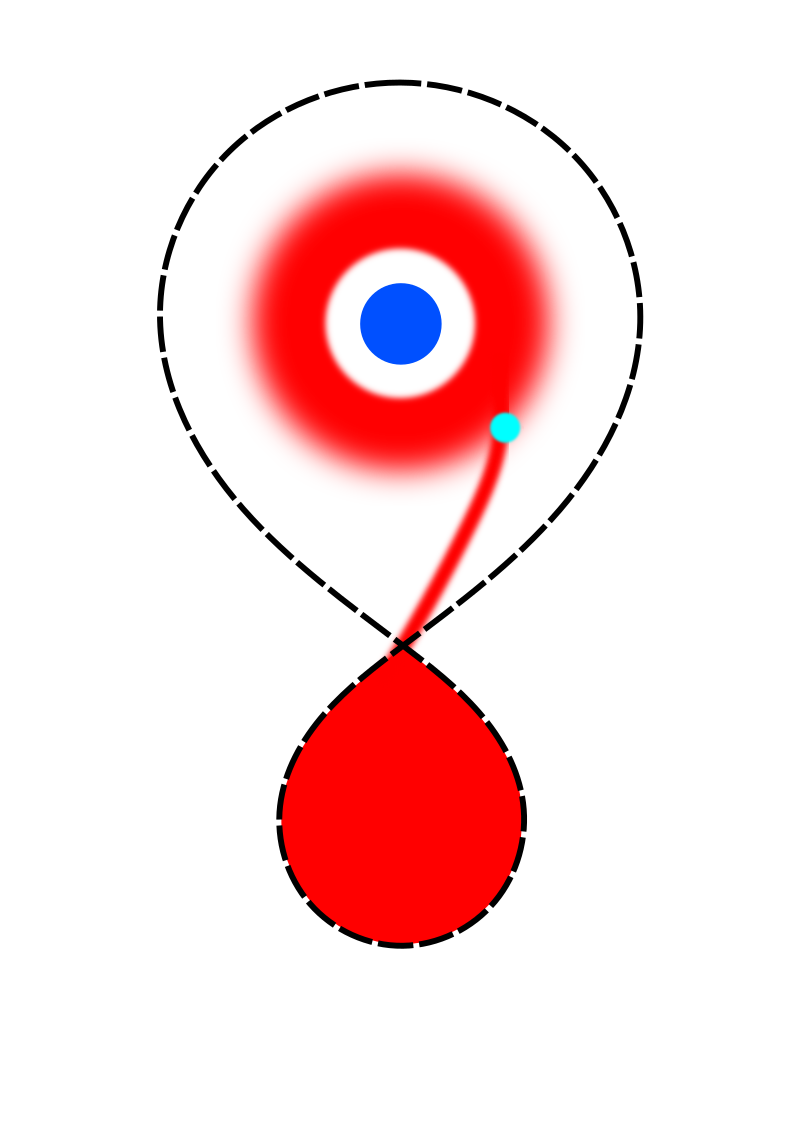
\includegraphics[width=0.6\textwidth]{figures/introduction/CV_schematic.png}
    \caption{A schematic of the structure of a CV, not to scale. The black dashed line outlines each Roche lobe . The dark blue circle is the white dwarf and is surrounded by its accretion disc. The lower red teardrop is the secondary star, and is connected to the donor via the mass stream. The light blue spot where the mass stream meets the disc is the bright spot impact region.}
    \label{fig:introduction:CV schematic}
\end{figure}

Systems actively undergoing mass transfer are important to our understanding of stellar evolution. A diversity of stars will experience a mass transfer phase, and losing mass strongly influences a stars' evolutionary path and must be accounted for. Of such systems, CVs in particular are interesting as modelling their eclipse lightcurves can yield precise, independant measures of both stars' mass and radius \citep{wood1986, Littlefair2008, Savoury2011}. Further, since the donor stars' evolution is completely dominated by its mass loss, CVs provide a window into binary evolution \citep{knigge2006}. The mass loss itself is driven by poorly-understood mechanisms, often attributed to magnetism and gravitational waves, that can also be probed using CV observation and modelling.
Since CVs are binary stars, they are open to comprehensive analysis, providing an excellent test-bed for binary modelling, and the difficult processes that contribute to them. Unfortunately, whilst semi-empirical modelling of most of the CV evolutionary track and population distribution is now possible \citep{Savoury2011,knigge11,Paxton_2015}, the field has yet to produce {\it physically motivated} models capable of accurately reproducing either the CV population distribution, or complete evolutionary track, indicating some shortfalls in our understanding. Of most significance to this work is the problem of missing Angular Momentum Loss (AML), where CVs with extremely low mass donor stars appear to be losing angular momentum much faster than our models predict \citep{wild2021}. This first chapter will summarise the current understanding of CV formation and evolution, and the current state of CV modelling. 

The bulk of this thesis is focused on two elements: firstly, the sample of well-characterised (i.e. measured masses and radii for both stars, white dwarf temperature and surface gravity, orbital period, and inclination) eclipse modelled CVs is small - only 18 systems prior to this work. I characterise an additional XXX systems\todo{Put in here how many systems}. While this is still a small sample, it is now enough for approximate statistical analysis. Second, using stellar models, I affirm the observations \citep{knigge2006,knigge11} that the canonical CV evolutionary track fails at periods shorter than $\sim 2.5$ hours, and produce an empirical correction to predicted AML, as a function of donor mass\todo{Hopefully!}. Through this, I hope to constrain the possible sources of missing AML. 


\section{Roche geometry}
\label{sect:introduction:Roche geometry}

Before discussing the formation, structure, and evolution of CVs, it is first critical to understand Roche lobes.
In a two-body orbital system, the Roche potential of a point is an effective potential in the non-inertial, co-rotating frame of reference. It is given by the sum of the gravitational potential energies due to the two masses, and the potential energy arising from centrifugal force. This can be described mathematically for each position vector:
\begin{equation}
    {\bf \phi} = -\frac{G M_1}{|{\bf r - r}_1|} - \frac{G M_2}{|{\bf r - r}_2|} - \frac{1}{2}({\bf \Omega} \times {\bf r})^2
\end{equation}
Where $\phi$ is the Roche potential, G is the gravitational constant, $\bf r$ is the position vector being considered, and $\bf \Omega$ is the angular momentum vector of the binary. $M_{1,2}$ and ${\bf r}_{1,2}$ are the masses and position vectors of the two orbiting bodies.

\begin{figure}
    \centering
    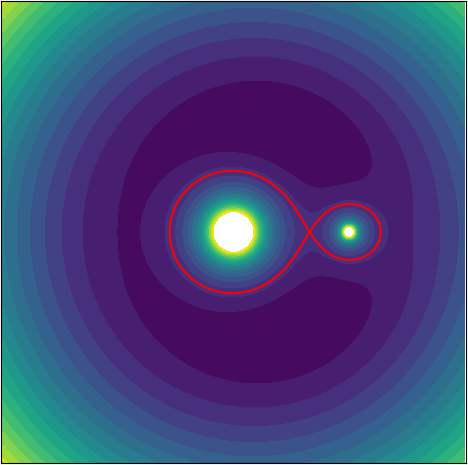
\includegraphics[width=.6\columnwidth]{figures/introduction/roche.png}
    \caption{Showing the Roche potential in the neighbourhood of the binary system, with the more massive primary star on the left. Darker regions are lower potentials. The red line illustrates the Roche lobes.}
    \label{fig:roche}
\end{figure}

Near to each of the bodies, the gravitational potential is large and negative, and dominates the Roche potential. This becomes \textit{less negative} as we move away from that body. Conversely, angular momentum is less negative closer to the center of mass, and more negative as we move away from the system and larger velocities are required to co-rotate. Broadly, there are then three regimes: a very negative Roche potential near each of the two bodies, a less negative region immediately surrounding the two bodies, and a very negative region far from the two bodies. The overall potential is smooth, so joining the three regions requires a ridge encircling the orbiting bodies, and a saddle between them. Figure~\ref{fig:roche} shows this graphically. The saddle is centred on the first Lagrangian point, $L_1$, and is the point at which a small (co-rotating) mass is attracted equally and oppositely by both bodies. We can trace the line of constant potential that passes through the $L_1$ point, giving two teardrops joined at the tips. The teardrop that encapsulates a star is known as its Roche lobe. Matter that extends beyond the Roche lobe is no longer gravitationally bound to its parent body, and will either fall onto its companion via the $L_1$ point, or otherwise be ejected from the star. This material will no longer be in a stable orbit, so will either be ejected from the system, or find a new higher orbit where the two-body effects are negligible.

The shape of the Roche lobes are non-trivial to calculate, and must be done numerically. However, approximations exist for the volume-equivalent radius of a Roche lobe (that is, the radius of a sphere of equivalent volume). Most commonly used is the \citet{Eggleton1983} approximation,
\begin{equation}
    \label{eqn:eggleton approximation}
    \frac{R_L}{a} = \frac{0.49 q^{2/3}}{0.6 q^{2/3} + \mathrm{ln}(1 + q^{1/3})}
\end{equation}
where $a$ is the orbital separation, and $q$ is the mass ratio of the system, $M_2 / M_1$. In CVs, where the secondary star is completely filling its Roche lobe, $R_L$ makes for a good approximation for the secondary stars' radius.


\section{Accretion in CVs}
\label{sect:introduction:accretion}
Accretion physics is important to the appearance and behaviour of a CV. While it is summarised here, more in-depth descriptions can be found in \citet{warner1995, hellier2001, ritter2010}.

When the donor star overfills its Roche lobe, matter is ejected from its surface at thermal velocities -- $\sim 10 \rm km\ s^{-1}$ for a 5000K M dwarf. This is small when compared to the orbital velocity of the system, and M dwarf velocities of $\sim 400-500 \rm\ km s^{-1}$ are common in the observations reported in \S\todo{Put this section in!}. Since the ejected material is effectively stationary as it leaves the donor, it falls along a ballistic trajectory towards the white dwarf primary and forms an accretion disc around it. 

Disc material gradually loses angular momentum and gravitational potential energy due to its viscosity, which acts over time to concentrate the majority of the disc's angular momentum in the minority of the disc's mass, ejecting some material at high velocities at the expense of moving the remainder closer to the white dwarf. This viscosity partially arises from friction within the fluid of the disc but the main source is thought to be from turbulence, random eddy currents moving material to different radii. This form of turbulence in a thin disc was formalised in the alpha disc model by \citet{shakura1973}, where viscosity, $\nu$, is related to scale height, $H$, and the speed of sound, $c_s$, by a free parameter, $\alpha$.
\begin{equation}
    \label{eqn:disc viscocity}
    \nu = \alpha c_s H
\end{equation}
Since turbulent eddies cannot be larger than $H$ or have velocities greater than $c_s$, $c_s H$ forms the upper limit of $\nu$, and $\alpha$ is limited in this model to values between 0 and 1. In typical CV accretion discs (i.e. quiescent discs, see \S\ref{sect:introduction:dwarf novae}), $\alpha$ takes values from $\sim 0.01 - 0.05$ \citet{hellier2001}.

Material that enters the disc must lose gravitational potential energy before it can be accreted to the white dwarf surface. Approximately half of this energy is lost thermally, through radiating accretion light, and the other half is converted to the kinetic energy necessary to maintain orbit about the white dwarf at lower altitudes. This low orbit has typical velocities roughly an order of magnitude higher than the rotational velocity of the white dwarf, so for material to settle on the stars' surface it must dissipate a large amount of kinetic energy. A region between the inner edge of the disc, and the surface of the white dwarf where this deceleration occurs is called the boundary layer, and can be a significant contributor to the total brightness of a CV. 

As the white dwarf is accreting material to its surface, one might expect it to grow in mass over time, and possibly even detonate as a Ia supernova as it crosses the $1.4 M_\odot$ Chandrasekhar limit. This postulation is supported by the white dwarfs in CVs being significantly more massive than their singleton counterparts \todo{ref}, but were this the case we would expect there to be a relationship between age, and white dwarf mass. \citet{McAllister2019} searched for this relationship, but found no correlation between the two, indicating that the white dwarfs in CVs do not grow over time, and are unlikely to reach the Chandrasekhar limit. Growth is thought to be limited by the accreted material cyclically detonating, in events called Classical Novae, outlined in \S\ref{sect:introduction:classical novae} \citep{Wijnen2015,sparks2021}. Serial detonation is even invoked as a potential source of AML, dubbed Consequential AML (CAML), that is described in \S\ref{sect:introduction:CAML}.



\section{CV variability and subtypes}
The sections above have outlined the general structure and evolution of a CV, but not all systems are well described by this picture. CVs exhibit significant variability even on human timescales, often on the order of several magnitudes in brightness. Further, a few subtypes of CV exist that either lie significantly outside the normal evolutionary tracks we expect, or contain exotic components. These are briefly discussed, though the focus of this work is on ``classic'' CVs, and the majority of these subtypes are fundamentally incompatible with our analysis techniques.

\subsection{Brown dwarf donors}
\label{sect:introduction:brown dwarf donors}

The formation channel of CVs does not require that the secondary star meets any minimum mass requirement, and it is theoretically possible to form a CV with a substellar brown dwarf donor \citep{politano2002,politano2004}. Because the donor is so small, these systems can form well below the period minimum, between 46 minutes and 2.5 hours \citep{politano2004}. CVs are observed with sub-minimum orbital periods, but observational evidence of these hosting brown dwarfs is rare. However, a few confirmations do exist, for example in SDSS J150722.30+523039.8 \citep{littlefair2007}

\subsection{Magnetic CVs}
\label{sect:introduction:magnetic CVs}

It is possible for white dwarfs to have very strong magnetic fields, in the region of tens to hundreds of megagauss. Such white dwarfs are called polars, and are an interesting field of study in their own right, but when a polar is accreting material from a donor star the system is designated as an AM Her star. The intense magnetic field strength alters the CV evolution in a two main ways. The strong field lines of the polar mean that the hot, charged photosphere material transferred to the primary cannot form an accretion disc and instead falls directly onto the surface of the white dwarf. The impacting material forms a bright spot on its surface, which is usually bright enough to be visible from earth. In addition, the strong field lines force the white dwarf to become tidally locked to the donor star. 

There is also a subclass of magnetic CVs with weaker field strengths of a few megagauss, known as DQ Her stars. In these systems, the white dwarf is not tidally locked, and a partial disc can exist. However, as the existence of a disc is crucial to the characterisation technique used in this work (see \S WHAT\todo{Put in the relevant section here} for details), magnetic CVs are unsuitable for our analysis.

\subsection{Helium-rich CVs}
\label{sect:introduction:AM CVn}

A small number of CV donors are helium-rich, with much smaller radii than their hydrogen-rich counterparts; these can be semi-degenerate helium stars, the cores of highly evolved main sequence stars, or a second white dwarf. The  As a CV donor must be in contact with its Roche lobe, such systems are far more compact than usual, with orbital periods $\lesssim 65$ minutes. Such systems are AM CVn stars, after the prototypical system AM Canum Venaticorum. For further discussion on AM CVn stars, see \citep{solheim2010}.

Early population studies expect that up to 50\% of CVs should host a helium white dwarf \citep{politano1996}, though to date this has been difficult to test. \citet{zorotovic2010} examined a sample of post-common envelope binaries and found only $13\pm7\%$ of the sample to be expected to evolve into a CV containing a helium white dwarf.


\subsection{Classical Novae}
\label{sect:introduction:classical novae}

The white dwarf in a CV is almost constantly accreting matter onto its surface. Over time this surface layer can build up, and get placed under immense pressure by the gravity of the white dwarf. Eventually, pressures rise enough to force material at the boundary to become degenerate, and once hot enough this boundary layer can begin nuclear fusion. 
Since the accreted material has become degenerate, it cannot expand in response to the extra energy from fusion and simply heats further, leading to more and more fusion and culminating in a complete detonation of the accreted material on the white dwarf's surface \citep{warner1995}. This detonation is finally able to overcome the surface gravity of the white dwarf, and the accreted material is blown from the surface.
These are generally one-off events, recognised by a significant brightening of the system of between 6 and 19 magnitudes, lasting anywhere from a few days, so several months. 

Once a system has experienced a classical nova, it is classified as a CNe system. \citep{warner1995}. However, theory suggests that all CVs experience classical novae many times over their lifetimes. The required amount of accreted material for the nova to occur depends on mass, but lies between $3\times10^{-5} M_\odot$ of hydrogen for a $1.3 M_\odot$ white dwarf, and $5\times10^{-3} M_\odot$ for a low mass, $0.6 M_\odot$ white dwarf \citep{hellier2001}. Typical CV accretion rates are around $10^{-9} M_\odot\ yr^{-1}$ for long period systems, and $10^{-10} M_\odot\ yr^{-1}$ for short period systems \citep{hellier2001, Pala2021}, suggesting classical novae recur at most every few million years, down to every few tens of thousands of years.

The amount of material retained by the white dwarf is likely negligible. Both population synthesis by \citep{Wijnen2015} and observations by \citep{McAllister2017} indicate no evidence of mass growth over time for the white dwarfs in CVs, and hence that the expulsion of the accreted material in a classical nova is complete.

A final note is that some CVs show multiple classical novae in relatively quick succession \citep{schaeffer2010}. These Recurrent Novae (RNe) are distinguished by having more than one observed nova event recorded. As good quality data only exist for the last few centuries, this enforces a soft limit on recurrence interval of a few hundred years, though recent efforts have been made to search ancient records for candidate events \citep{hoffmann2022}. Only a handful of confirmed RNe are known; the variable star index \citep{Watson2006} only contains 11 systems classified as RNe.

\subsection{Dwarf Novae}
\label{sect:introduction:dwarf novae}

CVs also undergo less extreme brightening events, called Dwarf Nova (DN) outbursts. These brighten the system by between 2 and 5 magnitudes \citep{warner1995} and are more brief than typical CNe, lasting less than $\sim 20$ days. However, in contrast to CNe, they have recurrence times much more in line with human timescales, ranging from a few days to some decades. This is due to the fundamental difference in the physical origin of the two phenomena.

DN outbursts do not originate directly from either star in the system, but rather from the accretion disc around the white dwarf. Such outbursts are well-described by the disc instability model \citep{cannizzo1993, dubus2018}.

Initially, the disc is in a cooler, ``low'' state with low temperature, low surface density, and low viscosity. Material in the disc moves inwards due to friction from turbulence (see \S\ref{sect:introduction:accretion}) which is relatively weak in the low viscosity material, so radial movement of disc material is slow.

If the accretion rate of donor material exceeds the rate material falls onto the surface of the white dwarf, then a buildup of matter begins in the disc, raising the density and temperature. Eventually, this annulus reaches $\sim 7000K$, at which point hydrogen becomes partially ionised and a rapid further increase in temperature is triggered as the material becomes optically thick and heat is trapped in the disc. In addition, as the temperature and density rise, so does $c_s$, and following Equation~\ref{eqn:disc viscocity}, so does viscosity, even assuming constant $\alpha$. In fact, $\alpha$ {\it rises} during outburst, to $\alpha \sim 0.1 - 0.5$ \citep{hellier2001}. This hot, luminous, ``high'' state is again stable, and the disc is said to be in outburst. 

Now that the disc is more viscous, material is moved inwards more readily. The infall rate onto the white dwarf is much increased, and is now higher than the mass transfer rate, so the disc is drained onto the surface of the white dwarf. As it does so, the surface density and temperature begin to fall, and eventually protons and electrons recombine into hydrogen. While recombination is an exothermic process, the release of energy is outweighed by the material once again becoming optically thin and allowing radiation to more easily escape the disc. The disc now quickly cools back down to the quiescent, ``low'' state, returning to a low surface density, and the cycle can repeat itself. For a more in-depth look at this model, refer to discussions by \citet{cannizzo1993}, \citet{osaki1996}, \citet{warner1995}, \citep{hellier2001}, and \citet{Hameury2002}.

Three types of DNe exist, which exhibit somewhat different behaviour than what is outlined above. The first of which are SS Cyg stars, distinguished by very consistent amplitudes across outbursts, though there is variation in length, shape, and recurrence time.

Z Cam stars exhibit standstills, events where the system enters outburst, peaks in brightness, then begins to dim. However, rather than returning to its quiescent magnitude, the brightness is maintained $\sim 1-1.5$ magnitudes below peak brightness for a long period of time, typically between a few days, and a few years \citep{simonsen2014}.

The third subtype are SU UMa stars. These systems are known for their more complex behaviour, exhibiting superoutbursts and superhumping, and are described in \S\ref{sect:introduction:SU UMa}

\subsection{SU UMa stars}
\label{sect:introduction:SU UMa}

SU UMa stars are distinguished by exhibiting superoutbursts, similar to the regular outbursts that the star still undergoes, but with greater amplitudes and durations, but longer recurrence times. These outbursts are triggered by the disc radius growing to such an extent that it becomes tidally perturbed by the donor star, and turns elliptical. This can only take place for when the donor star is less than $\sim 1/3$ the white dwarf mass, so only short period systems see these superoutbursts. \citep{hellier2001}. 
SU UMa stars are also known for their superhumping, which also arises from the disc eccentricity. The tidal interaction between the disc and the donor produces an area of increased luminosity at the edge of the disc between the white dwarf and the donor \citep{warner1988}. As the disc is elliptical, the distance between this disc edge and the donor varies over the course of an orbit, causing a similar variation in brightness as the donor moves around the disc.
These fluctuations are called superhumps, and are useful as they provide a diagnostic to the mass ratio for the system as the  \citep{Patterson1998, Patterson2001, patterson2005}. 

Because of the strong influence of the donor, the disc is also subject to precession, with a precession rate slightly longer than the orbital period. The superhump period, $P_{\rm hump}$ is then a combination of the orbital period, $P_{\rm orb}$, and the precessional period $P_{\rm pr}$,
\begin{equation}
    \frac{1}{P_{\rm hump}} = \frac{1}{P_{\rm orb}} - \frac{1}{P_{\rm pr}}
\end{equation}
and while $P_{\rm pr}$ is difficult to observe, both $P_{\rm orb}$ and $P_{\rm hump}$ can be readily observed with photometry from earth without the need for precise alignment that eclipse modelling requires. Since the precession period is dependant on the mass ratio and the disc radius, by finding the superhumping period of eclipsing CVs an empirical relationship can be found between the superhumping excess, $\epsilon$, and the mass ratio of a CV, where:
\begin{equation}
    \epsilon = \frac{P_{\rm hump} - P_{\rm orb}}{P_{\rm orb}}
\end{equation}
and several papers exist discussing and calibrating this relationship, see \citet{McAllister2019} for a recent calibration and good starting point for more information.


\subsection{Nova-like systems}

The disc instability model applies to CVs with mass transfer rates that are high enough to exceed the infall rate onto the CV during the ``low'' state, but low enough that the ``high'' state can still empty the disc. However, a subset of CVs have mass transfer rates high enough to sustain the high state and maintain a permanent outburst mode. Such systems are called Novalikes, or NL systems. Most NL CVs show little to no brightness variation, though a small number known as VY Scl stars do occasionally enter ``low'' states and dip in brightness by several magnitudes. \citet{livio1994} propose that this is triggered by a starspot rotating into the L1 point causing a fall in mass transfer rate. A precise mechanism here is not given, but since star spots are regions of concentrated magnetic fields, it is postulated that the stronger magnetic field of the spot disrupts magnetic braking in some fashion. A competing theory from \citet{wu1995} proposes that the fall in brightness is caused by the irradiation of the donor stars' atmosphere driving mass transfer, and that when this irradiation becomes blocked, the mass transfer rate falls enough for the disc to enter the low state for a short time.


\section{CV formation}
\label{sect:introduction:formation of CVs}

The formation of a CV begins with a binary system forming at a distance of $\sim 100{R_\odot}$. Crucially, the stars differ significantly in mass, one typically being $<1{M_\odot}$ and the other $>1{M_\odot}$ \citep{Ritter2012}. The lifespan of a star falls as its mass increases, so the larger star evolves faster than its companion, ascending the red giant branch after a few Gyrs and expanding to fill its Roche lobe. 
As the outer layers contact the Roche lobe, stellar material crosses the boundary between being gravitationally bound to the donor and being ejected from its surface. 
Once the outer layers of the primary contact the Roche lobe, the $\mathrm L_1$\ point forms a locus for mass to move from the massive, evolved star onto the less evolved secondary star.

As mass moves away from the primary, and away from the centre of mass of the system, it gains angular momentum. However, because angular momentum is conserved within the binary this is offset by a drop in separation, $a$, and the radius of the Roche Lobe, ${R_L}$, contracts. \textit{More} matter is now outside the primary Roche lobe, encouraging further mass transfer and hence further reduction in orbital separation \citep{Ritter2008}.

With this positive feedback loop, the primary can rapidly transfer its whole envelope, though the transfer rate $\dot M$ is too high to for all of this to be properly assimilated into the primary surface. The process is very rapid -- so rapid that models have been unable to properly resolve it, but is probably $\sim 10^2 - 10^3$ years in duration \citep{Ritter2012}. With this influx of mass, the secondary star grows and the accreted matter forms a thick, bloated, and deeply convective envelope on the star. The increased radius of the secondary brings the two bodies into contact \citep{Ritter2008} and the stars enter a common envelope phase of evolution. See \citet{paczynski1976} for an original reference on common envelope evolution, or \citet{ivanova2020} for a recent review of the topic. For detail on this phase as it relates to CVs, see \citet{taam1978, webbink1984, zorotovic2010, passy2011}.

The common envelope phase transfers much of the secondary stars' angular momentum to the shared envelope, though the mechanism for this is poorly understood \citep{demarco2011}. If the common envelope is substantial enough, the reduction in separation between the two stellar cores can be completely reduced, and the two merge together. If it is not, the entire envelope is stripped from the stars, and the two are left in a compact orbit. CV systems are the product of the latter scenario - the common envelope is ejected via a strong wind, leaving the remnant core of the primary as a white dwarf, and a low mass secondary companion M dwarf. 

The common envelope phase can be parameterised with the energies involved, namely the gravitational binding energy of the envelope, $U_{\rm bind}$, and the change in the angular momentum contained in the orbit before and after the common envelope phase, $\Delta U_{\rm orb}$, as the common envelope efficiency parameter, $\alpha$.
\begin{equation}
    \alpha = \frac{U_{\rm bind}}{\Delta U_{\rm orb}}
\end{equation}
This is known as the $\alpha$ formalism \citep{demarco2011}, and is a good illustration of how poorly we understand CE evolution. $\alpha$ should be a metric we can predict with models, but this has proven very challenging and several competing frameworks exist \citep{ivanova2020}. 

The energy needed to liberate the envelope is expected to come from the angular momentum of the binary, but some systems have been observed and characterised with $\alpha > 1$. suggesting that other sources, like the thermal output of the stars, can contribute to the envelope ejection \citep{demarco2011, ivanova2013}. Common envelope evolution remains a very difficult problem to solve, and only approximate models currently exist \citep{ivanova2020}, but the following scenario is generally accepted as likely in the case of CVs.

During the common envelope phase, the envelope is expelled into a planetary nebula \citep{Ritter2012}, and $\alpha$ in the case of a proto-CV hass been loosely estimated to be $\sim 0.2 - 0.6$ \citep{politano2007}, and some evidence exists for lower $q$ systems having larger $\alpha$ \citep{passy2013}. The ejecta carries with it angular momentum, causing $a$ to quickly fall from $\sim 100 R_\odot$ to less than $1 R_\odot$ \citep{Ritter2012}, leaving behind a white dwarf and a low mass companion star -- usually a cool, red M dwarf -- in an extremely compact orbit, typically a few \Rsun. At this point, the red dwarf detaches from its Roche lobe and mass transfer is shut off. Angular momentum is shed through magnetic braking and gravitational wave braking until the donor comes into contact with its Roche lobe. Mass transfer can then resume, though this time in the more stable secondary-to-primary direction. The system is now a CV, and its evolution from here will be dominated by AML and mass transfer, detailed in \S\ref{sect:introduction:AMLMechs}.



\section{CV evolution}
\label{sect:introduction:Summary of how AML and Mdot drive period evolution}

Initially, mass from the more massive star transferred to the smaller one, but once the system emerges from the common envelope phase, AML causes the orbit to tighten until the less massive red dwarf secondary fills its Roche lobe. This now means that mass transfer is moving matter closer to the system's centre of mass, imparting angular momentum to the secondary as it does so. This causes the donor to retreat, and increases $R_L$. Hence, mass transfer now acts to decrease further transfer \citep{Ritter2008}, rather than exacerbate it.

To resume mass transfer some mechanism is necessary to shed angular momentum and bring the secondary back in contact with its Roche lobe. 
Canonically, two mechanisms are thought to drive this; gravitational wave braking, and magnetic braking \citep{knigge2006,knigge11}.
AML drives the two bodies closer together and triggers mass transfer, and mass loss from the donor drives it to retreat from the white dwarf primary. These two processes find equilibrium when the donor is just barely overflowing its Roche lobe, and the angular momentum gained by the donor from mass transfer is offset by the AML from the system.
The mass transfer timescale of the donor is much shorter than its nuclear timescale, so mass loss dominates its evolution and gives rise to a single, unified CV evolutionary path.

There is a further complicating factor to consider; while the secondary is losing mass, it is not in thermodynamic equilibrium. The outer layers are being lost, which reduces the pressure on the core and so reduces the rate of fusion. 
Above masses of $\sim 0.1 M_\odot$, the thermal timescale is much longer than the mass loss timescale (this is later demonstrated in \S\ref{sect:method:evolutionary modelling}), so the star is unable to cool and contract to its equilibrium radius. This leaves the star hotter than it would be under zero mass loss, and its radius increased in response to the mass loss, proportionally to the mass loss rate \citep{knigge2006, knigge11}.


\subsection{The classical picture of CV evolution}
\label{sect:introduction:AMLMechs}

When two bodies orbit each other in space, the periodic warping of space-time produces gravitational waves \citep{einstein1918} and these waves carry energy away from the system, robbing it of angular momentum and reducing the orbital radius \citep{Paczynski1967}. In CVs, the rate of momentum loss from gravitational waves is small, so long timescales (by human standards) are needed to significantly alter the orbital period, $P$.
The rate of change of the period, $\dot P$, is possible to probe directly with medium-to-long-baseline observations (e.g. \citealt{qian2007, shafter2021}), but is a stochastic process and highly variable on observable timescales. However, this has not prevented some systems having their average $\dot P$ inferred indirectly and a few such characterisations have been done. 
Notably, \citet{pala2020} recently inferred the mass loss rates (which directly relates to $\dot P$) of 42 CVs from HST spectra, using the white dwarf temperature and mass as diagnostics. 
In the near future, CV gravitational waves are expected to be visible to the LISA mission, and direct measurements of $\dot P$ at scale will become feasible \citep{Meliani2000, kalomeni2016}. 

Population synthesis models do not match observations with gravitational braking alone, and magnetic braking is thought to make up the deficit (e.g. \citet{kolb1993a, kolb1993, Davis2008, garraffo2018}).
Additionally, \citet{Townsley2009}, \citet{Pala2021} infer the mass transfer rate (a diagnostic of $\dot P$) from the white dwarf surface temperature, and find results inconsistent with pure gravitational braking.

If one of the stars has a strong magnetic field (often assumed to be the secondary, though white dwarfs can have strong `frozen-in' magnetic fields \citep{TOUT2011}), any wind emanating from the system, which is made up of charged particles, and likely originating from the secondary, will couple with the magnetic field to some degree and carry some angular momentum away from the binary with it.
In the case of a CV, the wind originates from the secondary star and the magnetic field is often assumed to be associated with the secondary also, though white dwarfs can have strong `frozen-in' magnetic fields \citep{TOUT2011}.
A more detailed description of the modern understanding of magnetic braking is given in \S\ref{sect:introduction:magnetic braking}.


\subsection{Period evolution and key population features}
\label{sect:introduction:period distribution key features}
\begin{figure}
    \centering
    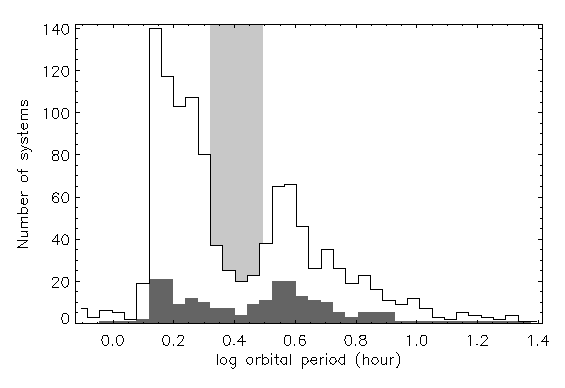
\includegraphics[width=\columnwidth]{figures/introduction/pd-rk.eps}
    \caption{Reproduced from \citet{southworth2015}, Figure~14. The orbital period distribution of RKCat \citep{RKCat} CVs identified by the SDSS (white histogram) and of the subset of these which are eclipsing (grey histogram). The light grey rectangle delineates the period gap at 2.1–3.1 hours. The periods have been collected into histogram bins which are of equal size in log space.}
    \label{fig:period hist}
\end{figure}

Through careful observation, The orbital period of a CV can be measured by tracking either their spectroscopic radial velocities (e.g. \citealt{gaensicke2009}), or the timings of repeating features in their lightcurves (e.g. \citealt{Littlefair2008}). Once this has been done for a large enough sample, a histogram of the periods can be plotted. This plot, shown in fig.~\ref{fig:period hist}, is important to understanding how a CV will evolve over time.
There are three immediately obvious features of the plot;
\begin{itemize}
    \item a long period cutoff, as the number of systems taper off after $\sim12$hrs
    \item a period gap at $\sim2-3$hrs
    \item a period minimum at $\sim1$ hour, with a pile-up of systems just above it.
\end{itemize}
Each of these features are discussed in turn.

\subsubsection{The period maximum}
\label{sect:introduction:period maximum}
In order for a system be be a CV, mass must be transferring from a less massive star, onto a compact object, constraining the maximum value of $q$ to $\sim1$, and demanding that the secondary extends out to $\sim R_L$. 

There are two immediately obvious constraints for a CV. The mass ratio, $q = \frac{M_{\rm donor}}{M_{\rm WD}}$, must be less than 1 for stable mass transfer, and the donor radius must be approximately equal to the Roche radius.
An additional constraint is that the maximum mass of a white dwarf is well known to be limited to $\le 1.4M_{\odot}$ before triggering thermonuclear runaway \citep{chandrasekhar1942}.

An important feature of a Roche lobe is that for a fixed mass ratio, $q=\frac{M_1}{M_2}$, its radius, $R_L$, is roughly linearly dependant on the orbital separation, $a$. Recall the Eggleton approximation for a Roche lobe radius, Equation~\ref{eqn:eggleton approximation}:
\begin{equation}
    \tag{\ref{eqn:eggleton approximation}}
    \frac{R_L}{a} = \frac{0.49 q^{2/3}}{0.6 q^{2/3} + \mathrm{ln}(1 + q^{1/3})}
\end{equation}

\citet{warner1995} found that the average density, $\rho_{av}$, for objects that fill their $R_L$ follows a robust relationship;
\begin{equation}
    \frac{\rho_{av}}{\rho_{\odot}} = 75.9 P_{orb}^{-2}(h)
\end{equation}
\citet{knigge11} derived a connection between CV secondary mass and radius, $M_2$ \& $R_L$. This can be manipulated to produce a mass-period relationship,
\begin{align}
    \rho_{av} = \frac{3 M_2}{4 \pi R_L^3} &\simeq 75.9 P(h)^{-2} \\
    \frac{R_L}{R_\odot} = C &\cdot \Big( \frac{M_2}{D \cdot M_\odot} \Big) ^{\alpha}
\end{align}
where $C$ and $D$ are constants for a particular regime, i.e., short-period, long-period, or period bouncer, and $\alpha$ is the mass-radius index \citep{Knigge2011b}.
Combining the above gives a pleasingly simple relationship.
\begin{equation}
\label{eqn:MP_relation}
    M_2^{(1-3\alpha)} \propto P^{-2}
\end{equation}

For long-period CVs, $\alpha = 0.67\pm0.04$ \citep{knigge11}, and equation \ref{eqn:MP_relation} becomes $M_2^{1.01} \propto P^{2}$, and larger secondary masses require longer periods. The theoretical maximum secondary mass of $1.4 M_{\odot}$ corresponds to a period of $\sim12$hrs, though in reality these higher masses are rarer and the frequency of CVs at these higher periods begins to drop much earlier, at $\sim6$hrs \citep{gaensicke2009}. Note while the above is specific to long-period systems, and $\alpha$ is a non-linear function of mass, and different values are needed for the period gap and short period regimes.


\subsubsection{The period gap}
\label{sect:introduction:period gap}

Between periods of around 2-3 hours, there is a dramatic fall in the number of CVs we detect. Volume-limited samples indicate that this is a real effect and not a selection bias \citep{Kolb1998}. However, the origin of this gap in the period is something of an open problem.

Models indicate that long period systems ($P > 3$h) have far higher mass loss rates than short period systems ($P < 2$h) \citep{ritter1985}. This suggests a significant change in braking mechanisms between the two regimes. 

The disruption of magnetic braking was proposed early on to explain the period gap \citep{rappaport1983, spruit1983}, and relatively shortly after \citet{kolb1993} showed more quantitatively that a sub-class of purely gravitational braking CV systems does not reproduce the observed population. 
Historically, the standard evolutionary path of CVs has involved the secondary becoming fully convective which was thought to disrupt the magnetic field and so cease MB \citep{knigge11}, though this mechanism has frequently been questioned. \todo{Gather references}

It is important to develop diagnostics for the nature of the period gap, and \citet{smith1998} show how spectral analysis could yield an accurate observed mass-radius relation for donor stars in CVs as evidence for MB, though they lacked the observations to apply their method. The mass-radius relation would later be carried out by \citet{knigge11}.
\citet{Davis2008} used population synthesis to demonstrate that, if the period gap is caused by disrupted MB, this may affect the mass function of quiescent CVs that are moving through the gap. They expect an excess of non-transferring CVs over low mass post-common envelope CVs that emerge from the common envelope phase directly into the period gap. These should form at a predictable rate across $q$, but due to the slow crossing of quiescent CVs, the latter `pile up' in the gap - a detectable effect observed by \citet{zorotovic2011}.

The system is still subject to gravitational radiation, however, so gradually evolves back towards shorter periods. Once the secondary reconnects with its Roche lobe, mass transfer resumes and the system again presents itself as a CV, emerging from the period gap at a $\sim2$hr period \citep{kolb2002}.

\subsubsection{The period minimum, and period bouncer systems}
\label{sect:introduction:period minimum and bouncers}

The period minimum was first predicted by \citet{rappaport1982}, and can be understood by considering the two governing timescales affecting the secondary. 
For donors with masses above $\sim0.1 M_{\odot}$, the donor is contracting in response to mass loss. 
As this proceeds, both $\tau_{therm}$ and $\tau_{\dot M}$ are increasing (the latter due to $\dot M_2 / M_2$ rising as the period shrinks). However, $\tau_{therm}$ rises faster, and at a period of $\sim80$ minutes \citep{ritter1998, McAllister2019}, $\tau_{therm}$ exceeds $\tau_{\dot M}$, causing the donor to lose mass adiabatically and expand rather than contract in respose to mass loss.
This allows the donor to remain in contact with its Roche Lobe when mass loss raises it to a higher orbit, and the system evolves to longer periods over time.

More quantitatively, as the components of a short period CV move closer together and the donor falls in mass, $\tau_{therm}$ and $\tau_{\dot M}$ become more out of balance, corresponding to $\alpha$ in equation \ref{eqn:MP_relation} decreasing \citep{Knigge2011b}. A main-sequence star will have $\alpha \sim 1$, but a secondary subjected to fast, adiabatic mass loss will have $\alpha \simeq -1/3$. Looking at the gradient of equation \ref{eqn:MP_relation}, the existence of a period minimum can be easily seen.
\begin{equation}
    \frac{\dot P}{P} = \frac{(3\alpha - 1)}{2} \frac{\dot M_2}{M_2}
\end{equation}
When $\alpha \le 1/3$, a negative $\dot M$ will produce a \textit{positive} change in $P$, and the donor begins to retreat from the white dwarf \citep{rezzolla2001}. 

This has been confirmed by \citet{knigge11}, who found that for period bouncer CVs, $\alpha = 0.21^{+0.05}_{-0.10}$, giving the following empirical version of equation \ref{eqn:MP_relation} in the post-period minimum regime.
\begin{align}
    M_2 \propto P^{-5.4}
\end{align}


\subsection{Problems with the classical picture}
\label{sect:introduction:modern AML}
A solid knowledge of exactly how and why CVs lose angular momentum has remained surprisingly elusive for several decades now. Early theories established gravitational waves and magnetic braking as the only two sources of AML \todo{ref}, but attempts to quantify this with evolutionary models \citep{knigge11} and population synthesis models \todo{ref} consistently fall short, as outlined in \S\ref{sect:introduction:AMLMechs}. Gravitational losses are well understood, and have been independantly observed and studied, but the sources and consequences of magnetism in a stellar context is not so easy. 

The spin rate and masses of CV donors is not seen in the singleton stars that are usually used to characterise magnetic braking \citep{rappaport1983,matt2015,garraffo2018a}. 
In addition, the disruption of magnetic braking is often motivated by the donor transitioning to a fully convective state, but X-ray emission level is a diagnostic of magnetic flux \citep{pevtsov2003}, and \citet{wright2016} found that the X-ray flux of CVs is similar between fully convective and non-convective main-sequence stars, implying a similar magnetic field strength. Furthermore, disagreement between observational and theoretical period gap and minimum locations \citep{knigge11} has left the disrupted MB model an area of active research. 
\citet{garraffo2018} recently proposed that the magnetic field does not weaken, but rather becomes more complex which reduces the efficiency of MB. This concept is discussed quantitavely in \S\ref{sect:introduction:Garraffo MB prescription}.


\subsection{The missing AML problem}

The evolution of CVs is driven by the donor stars. The orbital period is determined by the mass-radius relationship of the donor under mass loss, and the decay of the orbit should simply result directly from the two braking mechanisms (gravitational and magnetic). Figure~\todo{put in the one from my 2021 paper here} shows the relationship between the donor mass and orbital period, and the single unified CV track can be seen. Stellar evolution models can be built to try and reproduce this track, and indeed at long periods, our understanding of those mechanisms seem robust enough to produce models that satisfy observations. The period gap can, with some manual tweaks, also be reproduced with some accuracy. Unfortunately, at short periods ($\lesssim 2 hours$), the data begin to diverge from models. 

\S\ref{sect:introduction:Summary of how AML and Mdot drive period evolution} describes how the donor has its mass-radius relation altered by the presence of continued mass loss. The donor is larger than a singleton of the same mass, as the mass loss timescale is comparable to the thermal timescale and the donor is not quite able to maintain thermal equilibrium \citep{knigge11}. The degree of this inflation increases with more mass loss. As mass loss is driven by AML, it follows that a CV donor that has stronger AML will have a larger radius, and therefore sit at a longer period than a CV with weaker AML, altering the gradient of the tracks in Figure~\ref{fig:introduction:Knigge 2011 figure 9} at periods of $\lesssim 3h$. In this way, the shape of the tracks in Figure~\ref{fig:introduction:Knigge 2011 figure 9} is a diagnostic of the form of AML experienced by a CV across its lifetime \citep{knigge11}.
This also moves the period minimum to longer periods. The period minimum is caused by the donor's $\tau_{therm}$ becoming longer than $\tau_{\dot M}$, and since a faster mass loss will result in a shorter mass loss timescale, this crossover point is moved to higher masses and therefore longer periods. This is compounded by the faster mass loss resulting in more severe bloating of the donor star, so a donor of the same mass will connect to its Roche lobe at longer periods. 

\citet{knigge11} used took observations of donor masses and radii, with masses determined by either eclipse modelling, or the $\epsilon - q$ superhumper relationship, and radii are readily found from equating the donor radius to the expected Roche lobe radius. 
With donor properties for masses $\sim 0.1 - 1 M_\odot$, an unknown additional source of AML was added to their models, simply scaled relative to gravitational braking. This source is motivated by the disagreement between data and the model that omits this source. \citet{knigge11} find that the best-fit model to their data uses an excess braking that is $2.47 \times \dot J_{GR}$, where $\dot J_{GR}$ is AML due to gravity. Figure~\ref{fig:introduction:Knigge 2011 figure 9} is reproduced from their work, and shows the significant improvement in agreement with data.

\begin{figure}
    \centering
    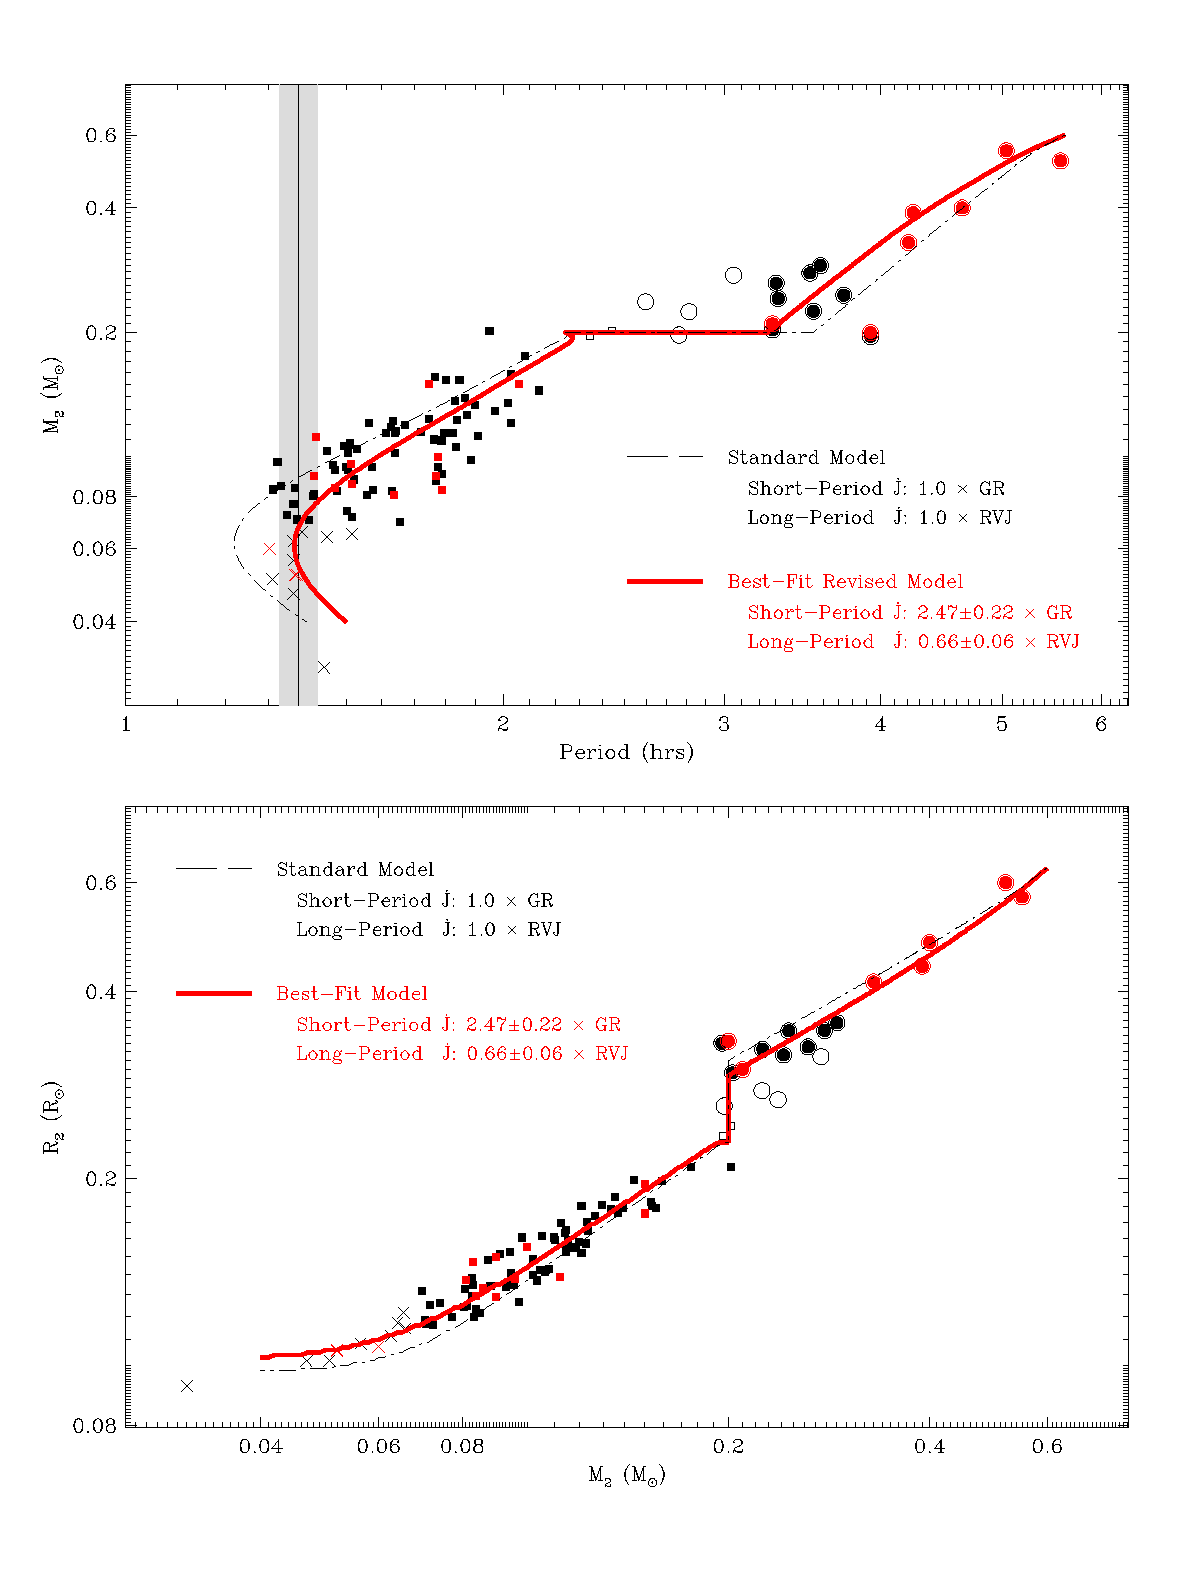
\includegraphics[width=\textwidth, trim={0 2cm 0 2cm}]{figures/introduction/Knigge11_fig9.pdf}
    \caption{Reproduced from \citet{knigge11}. {Black} markers are data from superhumpers, {Red} markers are data from eclipsers. {Crosses} denote candidate period bouncer CVs, {Squares} are short-period CVs, and {Circles} are long period CVs. {Open symbols} are omitted from their analysis due to lying in the period gap. The {Dashed Black lines} are their `standard', naiive model, and the {Solid Red line} includes an empirically determined excess AML source, scaled to gravitational wave braking. In the top panel, the {Vertical black line} signifies the observed period minimum, with the grey region as the FWHM of the period spike as measured in \citet{gaensicke2009}.}
    \label{fig:introduction:Knigge 2011 figure 9}
\end{figure}

\citet{Pala2017a} used the effective temperatures of the white dwarfs to probe CV evolution. The white dwarf temperature can be enhanced by accretion, so a hotter white dwarf suggests a higher mass transfer rate. This is sensitive to changes in $\dot M$ on short timescales, but still provides a valuable insight. \citet{Pala2017a} compare their white dwarf temperatures (and therefore mass transfer rates, and therefore AML rates) to MESA CV evolutionary tracks, and find that their observed temperatures are poorly described by only gravitational AML, but are more well-fitted by models that includes excess AML equivalent to gravitational losses, i.e. double-strength gravitational AML. Their analysis is useful but not wholly convincing, as the white dwarf temperatures are both quite poorly constrained, and sensitive to short-term variations in accretion rate that are known to occur\todo{cite}. In addition, the scaling of excess AML in relation to gravitational losses is not a free parameter in their analysis, and is only presented in the context of being obviously better by eye, rather than being tailored to the data.

The disagreement between theory and observation at short periods indicates that our understanding of AML in this regime is lacking, and a few proposals to rectify this have been suggested.

The obvious solution to the problem of missing AML is that we simply do not understand magnetism well enough to say that it ceases below the period gap. The donor may retain a residual magnetic field strong enough to drive some weaker form of magnetic braking that remains after the bulk of magnetic braking ceases. This is called Residual Magnetic Braking (RMB). Some evidence for RMB has been found in binary population synthesis models that focus on magnetic CVs \citep{belloni2020}. This approach asserts that a strong magnetic field from the white dwarf significantly reduces the effectiveness of magnetic braking by trapping a large fraction of the wind within the system, preventing it from carrying angular momentum away. The models that include this result in a better fit to key CV observables, specifically the orbital period distribution, white dwarf temperature distribution, and space density. While this theory does not apply to CVs in general, as the majority of systems do not have white dwarfs with strong enough magnetic fields, it has been suggested that a similar process could  occur on the donor \citep{garraffo2018}. 

The period gap is frequently attributed to the donor becoming fully convective, and this triggering a large reduction in magnetic field strength. However, observations of field M dwarfs of the same mass, with convective envelopes, are seen with key tracers of magnetism. Specifically, X-ray observations find that the coronal magnetic energy dissipation of fully convective stars is similar to non-convective stars \citep{wright2016}, and Zeeman-Doppler imaging of rapidly rotating M dwarfs indicate that the complexity of surface magnetic fields increases alongside rotation rate (e.g. \citealt{donati2003,donati2009,marsden2011,waite2011,waite2015}). Together, these observations strongly indicate that the disrupted magnetic braking model commonly accepted is ill-motivated, and may be more closely tied to field complexity than field strength \citep{garraffo2018}. If the gap is indeed driven by a sudden increase in field complexity, then it is reasonable to assume that magnetic braking remains significant after the system emerges from the period gap. However, this is not the only explanation for excess AML, and another strong candidate is consequential AML.


\subsection{Consequential AML}
\label{sect:introduction:CAML}

At its core, consequential AML (CAML) is a simple concept. It's known that the accreted material on CV white dwarfs detonates, and the majority of this material is lost from the system \citep{McAllister2019}. This will carry with it angular momentum, and so forms a third source of AML \citep{king1995,schenker1998}. By modelling CV evolution including this process, several issues of older CV population synthesis and evolutionary models can be solved at once \citep{Schreiber2016}. These issues are: 
\begin{enumerate}
    \item the observed mass of CV white dwarfs is systematically higher than singleton white dwarfs (e.g. \citealt{McAllister2019,pala2020});
    \item since the short period regime has much lower AML rates, CVs should spend most of their time below the period gap, and $\sim 99\%$ of CVs are expected to be short period \citep{kolb1993a}, but observations see a roughly even distribution between long and short period systems \citep{knigge2006};
    \item under purely gravitational losses, the period minimum was first calculated at $\sim 67$ minutes \citep{kolb99}, but is observed at $\sim 79$ minutes \citep{McAllister2019};
    \item the space density of CVs is roughly 1-2 orders of magnitude lower than population synthesis models predict.
\end{enumerate} 
The introduction of a modified, empirically calibrated CAML can account for these issues, making a compelling case for its validity. 

The maximum dynamically stable mass transfer rate of a CV is a function of $q$, related via the adiabatic mass-radius exponent, $\alpha_{ad}$, and the mass-radius exponent of the Roche radius, $\alpha_{L}$. Where the two intersect forms a threshold beyond which runaway mass transfer (much like the pre-CV common envelope phase) is triggered, and most likely results in a merger between the two bodies.
\begin{equation}
    \label{eqn:introduction:CAML stability threshold}
    \alpha_{ad} = \frac{{\rm d} ln(R_2)}{{\rm d} ln(M_2)}_{ad} = \frac{{\rm d} ln(R_L)}{{\rm d} ln(M_2)} = \alpha_L
\end{equation}
Where $\alpha_{ad}$ for convective stars is $-1/3$. Recalling the Eggleton approximation for the Roche radius, Equation~\ref{eqn:eggleton approximation}, we can find $\alpha_{ad}(q)$ \citep{Schreiber2016} in the absence of CAML,
\begin{equation}
    \alpha_{ad} = \frac{2}{3}\frac{ln(1+q^{1/3}) - \frac{1}{2}\frac{q^{1/3}}{1+q^{1/3}}}{0.6q^{2/3} + ln(1+q^{1/3})} (1 + q) + 2(q - 1) = -1/3
\end{equation}
Solving this equation gives a critical maximum value of $q < 0.634$. However, under the additional CAML, an extra source of $\dot J$ is introduced, $\dot J_{CAML}$.
\begin{equation}
    \frac{\dot J_{CAML}}{J} = \nu \frac{\dot M_2}{M_2}
\end{equation}
Here, $\nu = M_2^2 / (M_1(M_1 + M_2))$ and describes the angular momentum carried by ejected nova material, defined to be teh same as teh white dwarf momentum.
The right hand side of Equation~\ref{eqn:introduction:CAML stability threshold} is then altered by the increased AML rate.
\begin{equation}
    \alpha_{ad} = \frac{2}{3} \Bigg( \frac{ln(1+q^{1/3}) - \frac{1}{2}\frac{q^{1/3}}{1+q^{1/3}}}{0.6q^{2/3} + ln(1+q^{1/3})} \Bigg) + 2\nu + \frac{M_2}{M_1 + M_2} - 2
\end{equation}
The effect of this altered form of $\alpha_{ad}$ is that CVs with higher mass ratios are stable. Models with this prescription perform worse than non-CAML models. Binary population synthesis models by \citet{Schreiber2016} demonstrate that this model is not accurate to observations, producing {\it more} CVs with low mass donors than the non-CAML model. However, by altering the form of $\nu$ so that it is no longer tied to the white dwarf's angular momentum, a much better agreement with observations can be reached. This is the empirical CAML model, or eCAML.

$\nu$ is altered to a simple function of the white dwarf primary mass,
\begin{equation}
    \label{eqn:introduction:eCAML nu}
    \nu (M_1) = \frac{C}{M_1}
\end{equation}
where $C$ is an arbitrary constant chosen to best reflect observations, and \citep{Schreiber2016} adopt values of $C = 0.3 - 0.4$. The inverse relationship of more CAML at lower white dwarf masses is motivated by lower mass systems being able to retain less nova material, so more can be ejected and so carry more angular momentum. 

With eCAML, the dynamically unstable region \todo{put in their fig 1+2} is expanded. This has the important effect of making CVs with low-mass white dwarfs prone to dynamically unstable mass transfer, removing them from the CV population -- this simultaneously answers the question of CV white dwarfs being more massive than expected, and also vastly lowers the space density \citep{belloni2018}. Finally, the majority of systems that are now dynamically unstable are short-period CVs, so the observed period distribution is significantly more well-reproduced\todo{point at the Schreiber fig 2 panel}. 

Some observational evidence for eCAML has recently been uncovered by \citet{Pala2021}, where an inverse correlation between white dwarf mass and mass loss rate was observed. This is in line with Equation~\ref{eqn:introduction:eCAML nu}. 
Also, low mass ($< 0.5 M_\odot$) helium-core white dwarfs are expected to be formed in binaries, but are frequently observed as singletons. The merger scenario under eCAML provides a neat explanation for this \citep{zorotovic2017}
In addition to this, \citet{sparks2021} observed the spectra of CV donors and found significant non-solar abundances. This indicates that after nova outbursts, some of the nova-processed material is retained in the system long enough to be accreted onto the donor, and is supportive of lower mass white dwarfs having a lower eCAML contribution. In addition to supporting traditional eCAML this way, the re-accretion phase of the nova material provides a frictional AML mechanism \citep{Schreiber2016,sparks2021}, as the ejecta briefly forms a common envelope phase, as an alternative CAML mechanism to nova ejecta being completely lost from the binary. 


\subsection{Magnetic Braking}
\label{sect:introduction:magnetic braking}

Consider a blob of this charged wind material, moving with some sideways velocity in the plane of the orbit, almost certainly slower than the magnetic field lines. 
The blob will interact with the field and accelerated to co-rotate with them.
This higher velocity causes it to move outwards, to a higher orbit, where the field lines are moving even faster, accelerating the blob more. 
The wind then robs the star associated with the magnetic field of rotational angular momentum and its spin rate is slowed. The close proximity of the binary means that tidal effects are strong, and the donor is spun up again by robbing the orbit of angular momentum, reducing their separation and hardening the binary further \citep{verbunt1981}.

As an aside, \citet{wickramasinghe1996} presented theoretical motivation that CVs can have too strong a magnetic field to allow magnetic braking. Open field lines are necessary for wind to escape the system, so too strong a white dwarf magnetic field can trap the ionised gas in-system, suppressing the wind of the secondary. This Magnetic CV subclass is briefly described in \S\ref{sect:introduction:magnetic CVs}.

As the magnetic braking mechanism is a direct consequence of the donor star spinning down, the CV community is able to borrow insights from adjacent fields of study. The majority of M dwarfs experience some form of spin-down under magnetic braking \todo{cite this}, so observations of the magnetic field strengths of singletons should inform the efficacy of magnetic braking in CV binaries\todo{cite this}. Unfortunately, the typical CV rotational period is on the order of a few hours, and singleton M dwarfs are considered extremely fast rotators with periods of a day\todo{cite this}. Observations of singletons simply do not reach to the extremely low mass, rapid rotations that are frequently seen in CVs, so we are forced to rely on extrapolation and theory.

This carries with it some major practical issues. One is that while the broad effects of magnetic fields is relatively easy to intuit, quantitative physical understanding the mechanics and origins of magnetic fields is difficult, involving fluid dynamics, considering interactions with the accretion disc, and magnetism acting on large systems, which quickly become prohibitive to model and is usually handled with one of a variety of recipes. \citealt{knigge11} contains a detailed compilation of some older approaches, but the decade since has seen a few newer methodologies emerge. Here, two recent magnetic braking prescriptions are described in moderate detail: the \citet{matt2015} prescription, and the \citet{garraffo2018a} prescription. For a more complete, detailed summary of the modern understanding of M dwarf magnetic fields refer to \citet{kochukhov2021}. 


\subsubsection{Matt prescription for magnetic torque}
\label{sect:introduction:matt braking}

In \citet{matt2015}, an empirical prescription is derived that relates the torque felt by a low mass main sequence star to that stars' mass, radius, and Rossby number. The Rossby number is a fluid dynamics term for the ratio between the inertial and Coriolis force terms of the Navier-Stokes equations. A small Rossby number indicates a system dominated by Coriolis effects, and a large Rossby number indicates that centrifugal and inertial forces dominate. The Rossby number of a main sequence star can be calculated from $\Omega$, it's angular rotation rate, and $\tau_{\rm cz}$, the convective turnover timescale.
\begin{equation}
    \label{eqn:introduction:rossby number}
    {\rm Ro} = (\Omega \cdot \tau_{\rm cz})^{-1}
\end{equation}
Through the Rossby number, the effectiveness of magnetic braking is tied to rotation, which is extremely fast in CVs, and stellar mass and age, which affect $\tau_{\rm cz}$.

Their work makes use of observations of stars with masses less than $0.15 - 1.3 M_\odot$ and span ages of $\sim 10^{6-9}$ yrs, that have had their rotation periods measured. This dataset is used to calibrate a theoretically motivated empirical prescription for magnetic braking. There is some evidence for a saturation of magnetic activity below a critical Rossby value (a.k.a. above a critical rotational period) \citep{reiners2009}, where magnetic activity seems to no longer respond to changes in rotation. \citet{matt2015} adopt two generic relationships, 
\begin{equation}
    \bigg(\frac{B_*}{B_\odot}\bigg)^{4m} \bigg(\frac{\dot M_\omega}{\dot M_\odot}\bigg)^{1-2m} = Q \bigg(\frac{\rm Ro_\odot}{\rm Ro} \bigg)^{p}
\end{equation}
in the unsaturated regime, and 
\begin{equation}
    \bigg(\frac{B_*}{B_\odot}\bigg)^{4m} \bigg(\frac{\dot M_\omega}{\dot M_\odot}\bigg)^{1-2m} = Q \chi^{p}
\end{equation}
in the saturated regime. Here, $M_\omega$ is the global mass outflow rate, $B_*$ is the magnetic field strength at the stellar surface, and $M_\omega$ is the total mass outflow rate. The $m$ exponent is determined by the field geometry and wind acceleration profile, but functionally is a tuning parameter that likely falls in the range of $0.20 < m < 0.25$ \citep{matt2015}. The $p$ exponent encodes the dependence of magnetism on the Rossby number, $\rm Ro$, and is assigned as $p = 2$. $\chi$ is the inverse critical Rossby number for saturation, for which \citet{matt2015} adopt a value of $10$. $Q$ is a generic scale factor that the authors fit to observations.

The authors use these equations to eventually derive the spin rates for main sequence stars at some time $t$ after their initial spin period, $\Omega_i$, 
\begin{equation}
    \lim_{\Omega_* \gg \Omega_{\rm sat}} \bigg(\frac{\Omega_*}{\Omega_\odot}\bigg) \rightarrow \bigg(\frac{\tau_{\rm unsat}}{t}\bigg)^{\frac{1}{p}}
\end{equation}
\begin{equation}
    \Omega_* = \Omega_i \cdot e^{-t/\tau_{\rm sat}}
\end{equation}
for a rotation period of $\Omega_*$, and the threshold for saturation at $\Omega_{\rm sat}$. The two $\tau$ factors, $\tau_{\rm sat}$ and $\tau_{\rm unsat}$, are the spin-down timescales in the saturated and unsaturated regimes, and $\tau_{\rm sat} \ll \tau_{\rm unsat}$.

The authors take observations of two clusters, the $\sim 5$ Myr old ONC cluster and the $\sim 580$ Myr old Praesepe cluster, and use the first as initial conditions and the second as target distribution to reproduce. Figure~\ref{fig:introduction:Matt 2015 figure 2} is taken from \citet{matt2015}, and compares the initial and final conditions of their synthetic cluster model compared to these two boundary conditions. During the first few tens of Myrs of this model, the stars in the synthetic cluster are spun up as they contract, lowering their periods by factors of $\sim 5-10$. After this initial phase, which is much shorter than the spin down timescales, the more long-term spin evolution begins.

\begin{figure}[!tbp]
    \centering
    \begin{minipage}[b]{\textwidth}
        \centering
        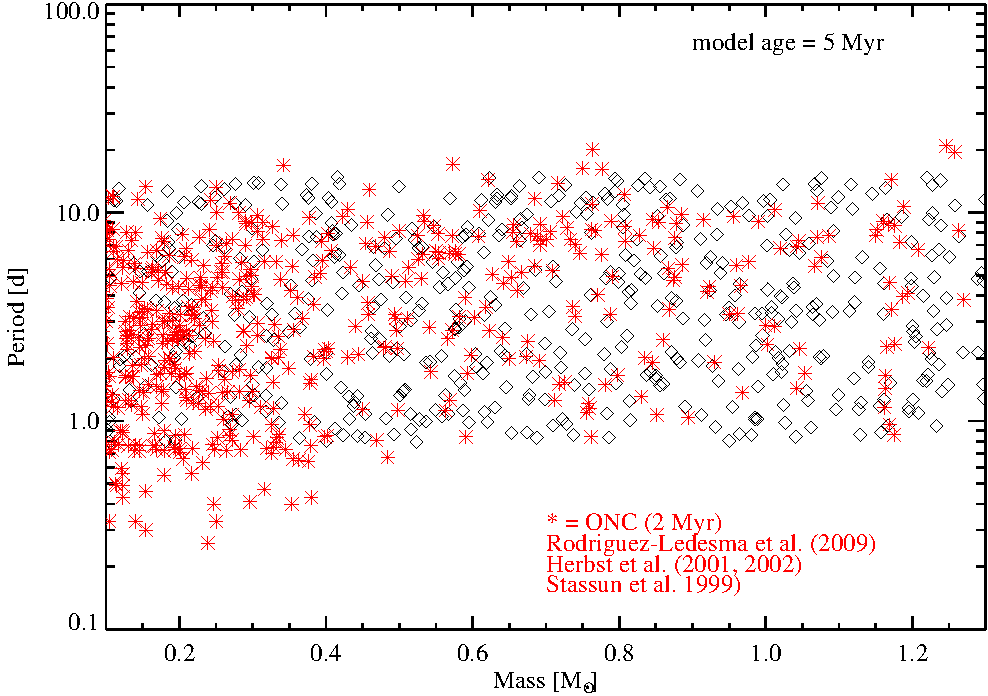
\includegraphics[width=0.8\textwidth]{figures/introduction/matt_2015_fig2a.pdf}
    \end{minipage}
    \begin{minipage}[b]{\textwidth}
        \centering
        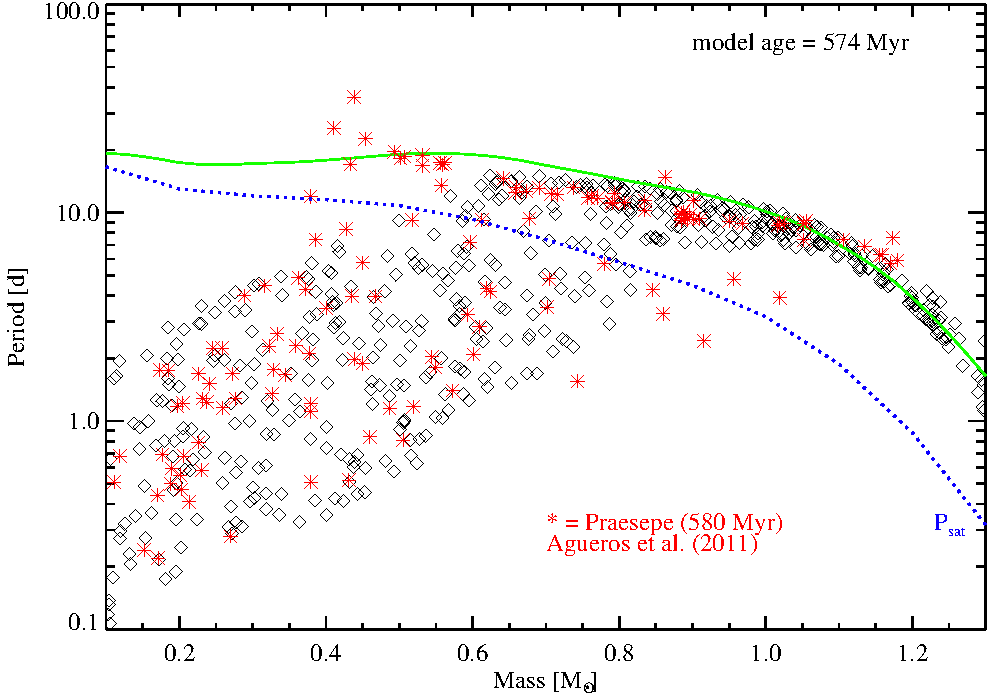
\includegraphics[width=0.8\textwidth]{figures/introduction/matt_2015_fig2b.pdf}
    \end{minipage}
    \caption{Figure taken from \citet{matt2015}. Red crosses are observations of the ONC ({\it top}) and Praesepe ({\it bottom}) cluster stars. Black diamonds are synthetic cluster stars. In the bottom panel, the solid green line is the theoretical asymptotic spin rate of unsaturated stars and the dotted blue line delimits magnetically saturated and unsaturated stars.}
    \label{fig:introduction:Matt 2015 figure 2}
\end{figure}

The agreement between the synthetic cluster and the Praesepe cluster at 574 Mrys is impressive. Above $\sim 0.8 M_\odot$, stars converge on a single narrow mass - period track just as is seen in the observations, and the large scatter below $\sim 0.8 M_\odot$ is also reproduced. Also, just as is seen in the cluster observations of Praesepe, the fastest rotators are those with the lowest masses. Both of these features arise from the transition from saturated braking, to unsaturated braking \citep{matt2015}. 

At formation, almost all stars are experiencing saturated magnetic braking. The single narrow track arises from higher mass stars spinning down faster than lower mass stars, bringing them down to the much less efficient unsaturated braking regime sooner. The pile-up of systems then produces the narrow track. The mass dependancy of this track comes from the fact that $\tau_{unsat}$ is shorter for lower mass stars.
The broad population of low mass rapid rotators is a direct result of the broad initial conditions, which span an order of magnitude themselves, and the longer spin-down time of lower mass stars in the saturated regime allowing them to remain at high rotation rates for longer. 

However, this model does fail in a few key respects. In the right panel of Figure~\ref{fig:introduction:Matt 2015 figure 2}, a small population of very slow rotators can be seen at $\sim 0.4 M_\odot$. The slower rotation rates of these stars suggests an alternative spin-down mechanism. The inverse problem is seen at $\sim 0.7 M_\odot$, where a handful of stars are seen rotating {\it faster} than predicted by any of the synthetic cluster stars, suggesting that magnetic braking is not as effective in their case.
More importantly for the CV field, the parameter space of CVs is completely uncovered, as CVs have rotation periods of $< 0.2$ days on the high end, and the systems that this work concerns have periods of $\lesssim 0.07$ days. While this would firmly place CVs in the saturated regime, there is evidence of a `supersaturated' regime at extreme rotation periods that may be relevant to CV donors \citep{James2000, Wright2011, Argiroffi2016}. This possibility is also noted by \citet{Gossage2021} when outlining best practice use of this prescription in the stellar evolution code MESA, though the subject is not a settled matter and competing evidence for the {\it lack} of supersaturation has been reported by \citet{jeffries2011}.


\subsubsection{Garraffo prescription for magnetic torque}
\label{sect:introduction:Garraffo MB prescription}

The \citet{garraffo2018a} model considers the morphology of the magnetic field to also be important the the strength of magnetic braking, based on the work by \citet{garraffo2015}. The primary justification for this inclusion is observations of open clusters of a known age, where a bimodality is seen in the rotation rates of stars of similar masses\todo{Cite skumanich gap}. Some stars appear to be fast rotators, and some are slow rotators, and there is a dearth of systems between the two. 
Previous attempts to model this bimodality have relied on a random, unexplained transition between an efficient braking state, and an inefficient braking state \citep{spada2011,reiners2012, gallet2013}, and \citet{garraffo2018a} expand on this by offering a shift in magnetic field morphology as the underlying trigger.

Their formalisation of this is based on two assumptions. They assume that stars with the dipolar component of the magnetic field dominating  follow a known spin-down law, with a mass dependence reflecting $\tau_{\rm cz}$\todo{cite Skumanich}. Second, they assume that there is some relationship between field morphology and stellar spin rate. Specifically, that stars rotating more rapidly have more complex magnetic fields. This is formalised via an AML rate, $\dot J$,
\begin{equation}
    \dot J = \dot J_{\rm dipole}Q_J(n)
\end{equation}
where $\dot J_{\rm dipole}$ is the dipole loss under the Skumanich law, $\dot J_{\rm dipole} \propto \Omega^3 \tau$. $Q_J$ is a modulating factor that encapsulates the field complexity at the stellar surface, and is controlled by the complexity factor, $n$, which has its own prescription. \citet{garraffo2016} derive an equation for $Q_J$, based on fitting the results of simulations with varying field complexities.\todo{Explain the model, and the origin of these numbers before reporting the relationship}
\begin{equation}
    \label{eqn:introduction:garraffo complexity modulation}
    Q_J(n) = 4.05 e^{-1.4n} + \frac{n-1}{60Bn}
\end{equation}
Where $B$ is the magnetic field strength at the stellar surface. As the second term is only significant for $n > 7$, \citet{garraffo2018a} consider $n = 7$ as the maximum complexity, consider only the first term of this relation. This is the equivalent of the saturation of magnetic braking from \S\ref{sect:introduction:matt braking}, but here is contingent on field complexity rather than $\rm Ro$. 

\citet{garraffo2018a} suggest the following relation between $\rm Ro$ and $n$,
\begin{equation}
    \label{eqn:introduction:garraffo field complexity}
    n = 1 + \frac{0.02}{\rm Ro} + 2 {\rm Ro}
\end{equation}
based on observations of open clusters. The three terms reflect three aspects of the magnetic braking model - the minimum complexity is defined as $n \equiv 1$, the first factor encodes stars with small $\rm Ro$ having large $n$ (e.g. young, fast rotators), and the third term gives stars with large $\rm Ro$ similarly large $n$. 
This prescription means that the AML of a star is purely a function of its Rossby number, c.f. Equation~\ref{eqn:introduction:rossby number}.

Similarly to \citet{matt2015}, \citet{garraffo2018a} run a population synthesis model to compare to observations using initial conditions taken from the 13 Myr old h Persei cluster \citep{moraux2013}, but the authors show that differences between alternative initial conditions do not survive longer than 200 Myrs. Observations of stellar rotation periods and colour from several clusters with known ages are then compared to the synthetic population.

The resulting distribution does recover the Skumanich bifurcation observed in open clusters, reproducing the fast and slow rotating populations and the gap between them, though the large uncertainty in the age of the cluster does introduce some discrepancy. 
In addition, the synthetic cluster does not consider the effects of close binary stars, which will affect the spin-down rate through tidal effects. As the comparison to data is done with color, filtering out binaries is difficult. However, this effect is ignored by the author, as there is evidence that the binary fraction in open clusters is low \citep{meibom2007}.
The mass dependency of this track is also reproduced by the model, and Figure~\ref{fig:introduction:garraffo 2018a fig 4}.

\begin{figure}
    \centering
    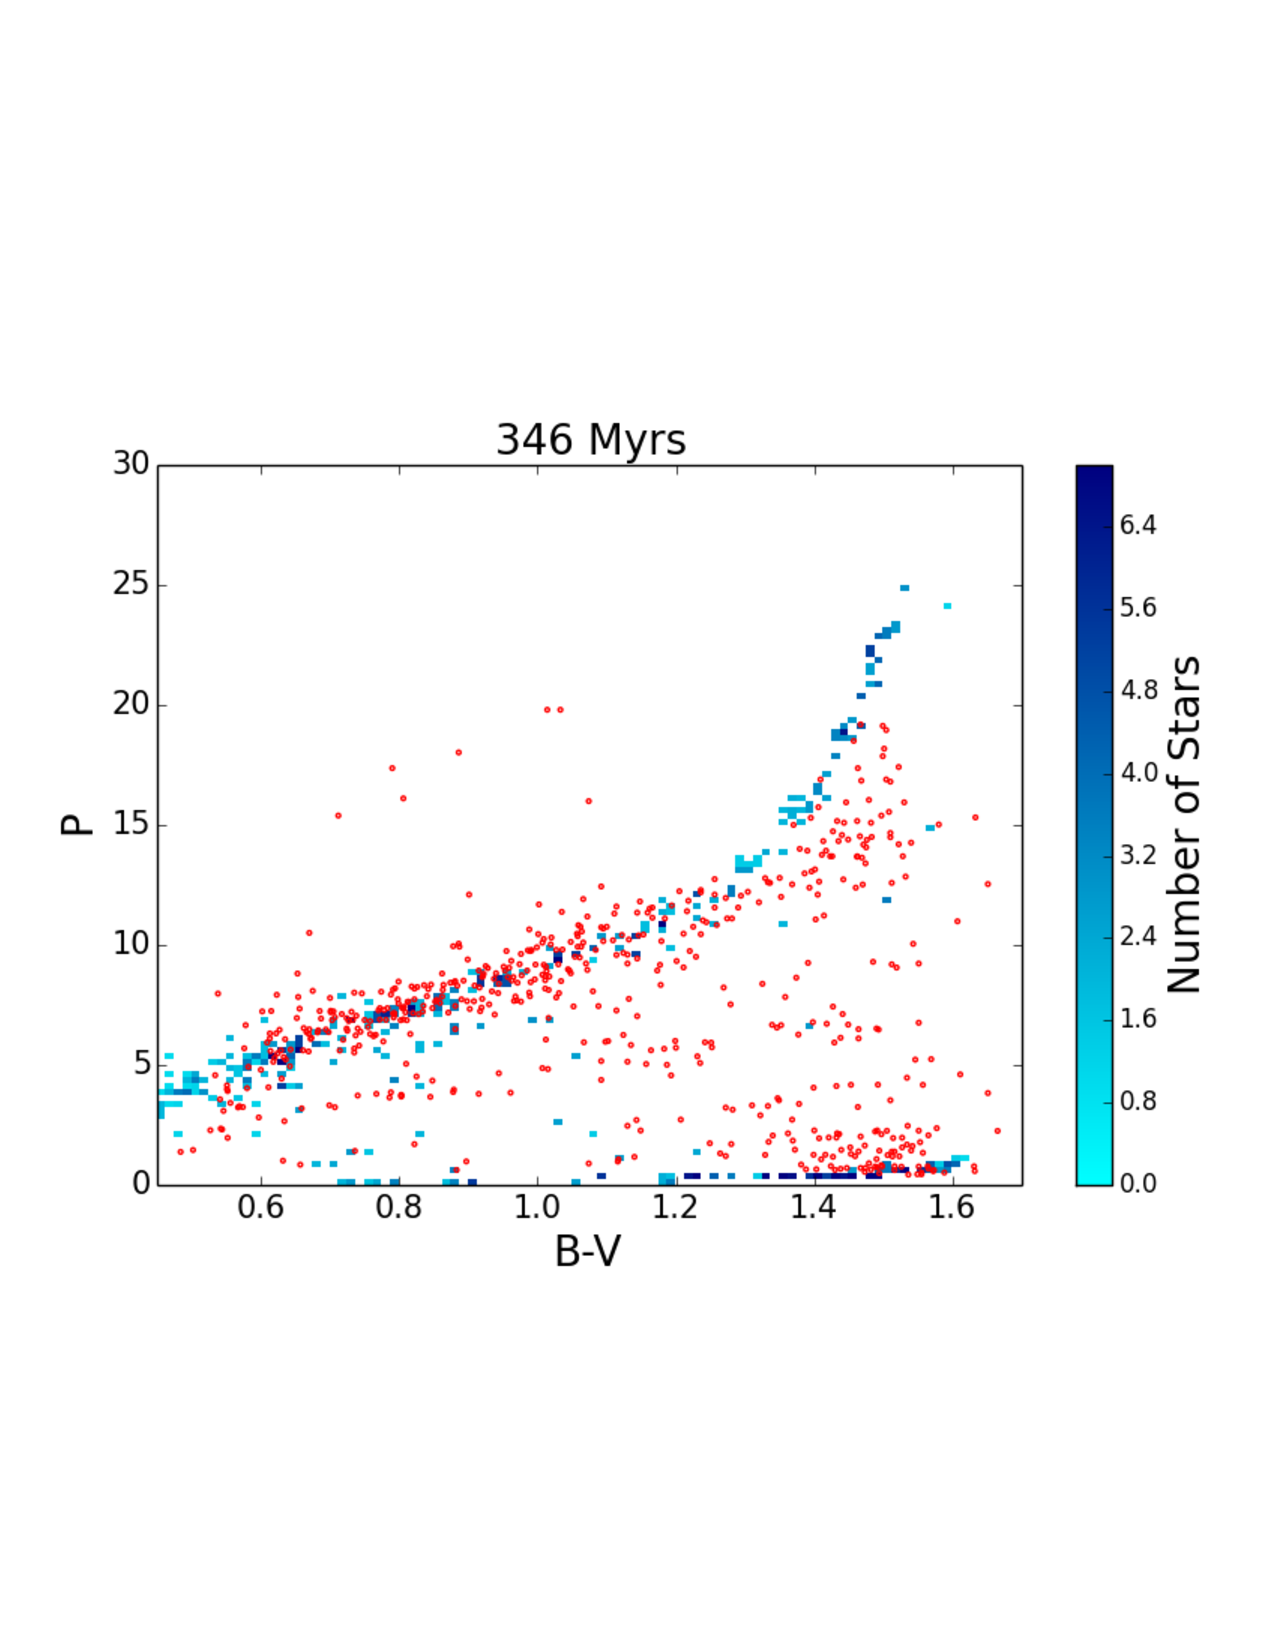
\includegraphics[width=0.8\textwidth, trim={0 5cm 0 5cm}]{figures/introduction/garraffo2018_M37_346_hPer.pdf}
    \caption{Example comparison between synthetic and observed cluster populations taken from \citet{garraffo2018a}. Red points are observations of M37, which has its age measured at $\sim 346 - 550$ Myrs. Blue points are the probability distribution of the synthetic cluster population from \citet{garraffo2018a}.}
    \label{fig:introduction:garraffo 2018a fig 4}
\end{figure}

The \citet{garraffo2018a} prescription is simpler in concept than the \citet{matt2015} prescription, and both prescriptions perform well. However, neither formulation covers the parameter space of CV donors, and both are semi-empirical with some arbitrary decisions made in order to fit data. This makes both approaches highly vulnerable to extrapolation errors and difficult to trust in the context of CV evolution, especially in the short period regime.


\subsubsection{Comparisons to the Rappaport, Verbundt and Joss model}

We can examine the differences between these prescriptions in the case of CV evolution by applying them to a donor evolutionary track, and \citet{knigge11} has constructed a donor sequence using their own models that reasonably accurately reproduces observations. The masses, radii, and periods along the sequence are given, so the would-be effects of the magnetic braking prescriptions described above can be calculated. In addition to the two previously discussed prescriptions, the default MESA \citep{Paxton_2015} magnetic braking prescription \citep{rappaport1983} is included. This prescription includes a magnetic braking index, $\gamma$,
\begin{equation}
    \dot J = -3.8\times10^{-30} M R_\odot^4 \bigg( \frac{R}{R_\odot} \bigg) \omega^3
\end{equation}

Note that in the specific case of CVs, period and radius are synonymous with one another, due to the requirement that the donor is in contact with the Roche lobe, and is tidally locked. 

\begin{figure}
    \centering
    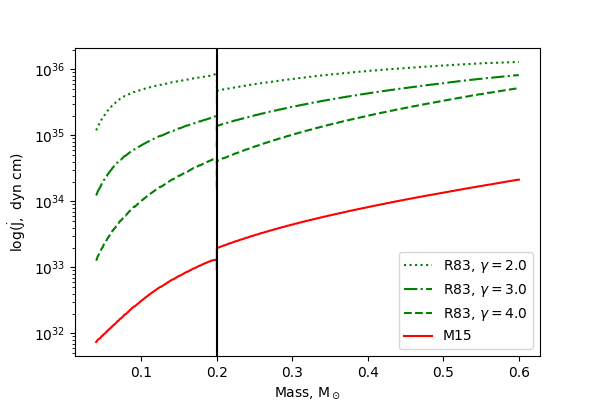
\includegraphics[width=\textwidth, trim={1cm 0 0 0}]{figures/introduction/rappaport_matt_magbraking.png}
    \caption{Showing the AML rates, $\dot J$, of three magnetic braking prescriptions, applied to the masses, radii, and spin periods of the `standard' CV donor track of \citet{knigge11}. The vertical black line shows the mass at which \citet{knigge11} enforces the period gap to occur. {\bf Green lines} show the \citet{rappaport1983} magnetic braking prescription, which is the default used in MESA \citep{Paxton_2015}. The {\bf red line} shows the \citet{matt2015} prescription.}
    \label{fig:introduction:rappaport garraffo matt magnetic braking}
\end{figure}

Figure~\ref{fig:introduction:rappaport garraffo matt magnetic braking} shows how the \citet{matt2015} magnetic braking prescription compares to the default MESA mabgnetic braking prescription, from \citet{rappaport1983}. 

The differences between the three prescriptions is clear in both the overall strength of the prescriptions, but also in how they evolve with mass. All the prescriptions shown decrease at lower masses, but at different rates. In the context of CV evolution, a different dropoff rates of magnetic braking would alter the shape of the donor mass-radius sequence, so observations of CV donors should be able to allow us to evaluate the effectiveness of different braking prescriptions.



\section{This work}
\label{sect:introduction:this work}